%!TEX root = ../fbi.tex

\section{Entanglement spectrum}
\label{sec:ES}

The quasi-1D cylinder geometry is also convenient for calculating the 
entanglement spectrum for entanglement cuts transverse to the 
cylinder. The procedure for computing the Schmidt decomposition is the 
same as for a MPS, and implies a canonical form for the quasi-1D MPS

$$
\ket{\psi} = \sum\limits_{\{p_i\}} \Gamma_{p_1} \Lambda \Gamma_{p_2} ... \Lambda \Gamma_{p_N} \ket{p_0 p_1 ... p_N}.
$$

The elements $\lambda_i$ of the diagonal matrix $\Lambda$ which 
appears in the canonical form,
are related to the non-zero eigenvalues $\rho_i$ of the reduced 
density matrix for the left or right half of the system via $\rho_i = 
\lambda_i^2$.

The entanglement spectrum $\epsilon_i$  is defined via the equation 
$e^{-\epsilon_i} = \rho_i$. One says that the entanglement spectrum 
are eigenvalues for the entanglement Hamiltonian $H_e$, where 
$e^{-H_e} = \rho$ is the reduced density matrix for the half-infinite 
cylinder on one side of the entanglement cut. 

Despite the infinite size, information about the entanglement 
Hamiltonian eigenstates can be extracted from the MPS procedure as 
well. The tensor network structure provides an effective reduced 
density matrix $\tilde{\rho}$ and entanglement Hamiltionian 
$\tilde{H_e}$ that are unitarily related to $\rho$ and $H_e$, but that 
acts on each virtual index crossed by the entanglement cut. The 
eigenstates of this Hamiltonian carry quantum numbers for each 
symmetry respected by the cut - in our case charge and momentum 
parallel to the cut - that match the corresponding Schmidt states. We 
will further discuss how the charge is assigned to edge states in 
section \ref{sec:symmetry}, and in section \ref{sec:perturbations}, we 
will see that the entanglement eigenstates can be related to edge 
states for the MPS parent Hamiltonian with open boundary conditions. 

\brayden{Something about history of 2d SPTs having gapless 
entanglement edges. Possibly see brayden's advancement talk.}
Gapless entanglement spectra have been shown to be robust features of two-dimensional topological and symmetry protected topological (SPT) phases.

\begin{figure}[htbc]
	\centering
	\includegraphics[width=\columnwidth]{{EntanglementSpectrum_L10.pdf}}
	\caption{Entanglement spectrum on a zig-zag edge L=10 cylinder}
	\label{fig:ESL10}
\end{figure}


\begin{figure}[htbc]
	\centering
	\includegraphics[width=\columnwidth]{{EntanglementSpectrum_L9.pdf}}
	\caption{Entanglement spectrum on a zig-zag edge L=9 cylinder}
	\label{fig:ESL9}
\end{figure}


The entanglement spectra on cylinders with even and odd width circumferences 
are shown in \ref{fig:ESL10} and \ref{fig:ESL9}. We find that the entanglement 
spectrum looks like it has a gapless edge mode with linear dispersion near 
momentum zero. In figure \ref{fig:EEScaling}, we compare the lowest points in 
the spectra for several cylinder widths. The finite size scaling confirms that 
the entanglement gap closes as $1/L$, as you would expect for a gapless mode 
with linear dispersion.

\begin{figure}[htbc]
	\centering
	\includegraphics[width=\columnwidth]{{EntanglementEnergyScaling.pdf}}
  \caption{Power law fits for the lowest five states above the ground state in Figure \ref{fig:ESL10}. The 
  $1/L$ scaling is a signature of a gapless (entanglement) Hamiltonian. Due to the small system size, 
  points at non-zero momentum still deviate significantly from $1/L$ scaling.}
  \label{fig:EEScaling}
\end{figure}

The most likely explanation for this gapless edge mode is that the state has 
topological or SPT order. By computing the topological entanglement entropy, 
as shown in \ref{fig:TopologicalEE}, we can rule out 
topological order for this state. Combined with the vanishing of topological 
entanglement entropy, these spectra suggest that the 
HFBI state are in a featureless SPT phase. However, we are still lacking 
several pieces of evidence for this claims. In order to prove that the state 
is truly featureless, we need to find a local parent Hamiltonian that has the 
HFBI as its unique, gapped ground state. We need to decide which subgroup 
(or subgroups) $G$ of the wavefunction's symmetries can be used to protect the 
SPT phase, and then test this by perturbing the parent Hamiltonian.

\begin{figure}[htbc]
	\centering
  \includegraphics[width=\columnwidth]{{TopologicalEntanglementEntropy.pdf}}
	\caption{The topological entanglement entropy $\gamma$ is consistent 
	with 0.}
	\label{fig:TopologicalEE}
\end{figure}

Of course, diagonalizing interacting 2D Hamiltonians is hard. We'll work up to 
these claims not by searching all possible Hamiltonians for a parent, but by 
looking more closely at the entanglement spectra.

Notice that many points in the spectrum are doubly degenerate - those that are 
assigned a non-zero $U(1)$ charge - and on odd circumference cylinders, the 
entire entanglement spectrum is doubly degenerate, a property shared with 1D 
SPTs. This suggests that the the HFBI state as a 1D state with any  
fixed odd cylinder circumference $L$ is a 1D SPT. We will discuss in
Section \ref{sec:symmetry} how to explain the degeneracies in these spectra 
using the action of the symmetry on the edge, and how to prove that the odd 
circumference cylinder states are indeed 1D SPTs while the even circumference 
cylinder states are not. This will shed light on what the appropriate symmetry group to use.

Given that only odd circumference cylinders are SPTs, one might wonder whether 
odd and even $L$ cylinders approach two differt phases in the thermodynamic 
limit. In Section \ref{sec:CFT}, we will provide evidence against that 
possibility, by showing that in both cases, the low-energy, linear dispersing 
part of the entanglement spectra can be described by the same conformal field 
theory. Thus, in the thermodynamic limit, the two edge spectra approach the 
same set of points.
	
\subsection{Symmetry action on the edge}
\label{sec:symmetry}

Similarly to the above calculations, we treat the HFBI wavefunction on a 
cylinder of a fixed circumference $L$ as a matrix product state, and use the 
method of \onlinecite{pollmann2010} to determine the action of the symmetry on 
the virtual legs of the tensor network.

Each on-site symmetry of the wavefunction $U_g = \otimes_i u^i_g$, with $U_g 
\ket{\psi} = e^{i \Theta_g} \ket{\psi}$ is assigned an operator $V_g$ that 
acts on the virtual leg of the MPS, that satisfies the equation pictured in 
Figure \ref{fig:mps_group_sym}. For an MPS with a nondegenerate largest 
transfer matrix eigenvalue, this equation is guaranteed have a unique solution 
for $V_g$. By combining $N$ such blocks together and connecting them with 
periodic boundary conditions, we recover the fact that $U_g 
\ket{\psi} = e^{i \Theta_g} \ket{\psi}$, with $\Theta_g = N \theta_g$, since 
all of the $V_g$ and $V_g^{\dagger}$s cancel pairwise.      

\begin{figure}[htbc]
    \centering
    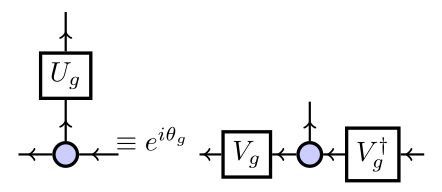
\includegraphics[width=0.6\columnwidth]{group_sym.png}
    \caption{Matrix Product State symmetry \brayden{fix to use canonical form}}
    \label{fig:mps_group_sym}
\end{figure}

In general, the $V_g$ do not have to form a linear representation of the 
group, but could instead be a projective representation. This can be explained 
in the MPS language as follows: if instead the blocks are connected together 
with different boundary conditions, as in Figure \ref{fig:mps_boundary}, we 
discover that $U_g$ transforms $\ket{\psi}$ to a similar state with 
transformed boundary conditions, $B \rightarrow V_g^{\dagger} B V_g$. This 
action on $B$, one can show, is a group representation.

For open ends - if $B$ factors into left and right parts, $B = 
\vket{b}\vbra{b}$ - the action of the symmetry on the boundary can also be 
factored, $\vket{b} \rightarrow V_g \vket{b}$. This action does not have to be 
a group representation, but can fail up phases $V_g V_h = e^{i \omega(g, h)} 
V_{gh}$.  

\begin{figure}[htbc]
    \centering
    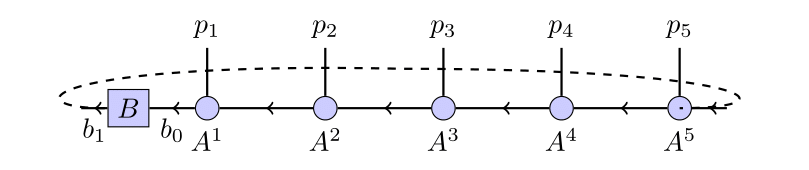
\includegraphics[width=\columnwidth]{mpsbc.png}
    \caption{Matrix Product State with arbitrary boundary conditions}
    \label{fig:mps_boundary}
\end{figure}

An extension of this to treat inversion symmetry is explained in 
\onlinecite{pollmann2010}. It works identically, but instead each matrix 
product state is transposed in the basis \brayden{Add pictures for inversion 
symmetry in MPS}.

\begin{tabular*}{\columnwidth}{@{\extracolsep{\stretch{1}}}*{5}{r}@{}}
\toprule
$\mathbf{G}$ & $\mathbf{U_g}$ & $\mathbf{\theta_g}$ & $\mathbf{V_g}$ &$\mathbf{V_g V^*_g}$ \\
\midrule
 $U(1) $ & & & & \\
 $\mathcal{\pi} \mathcal{I}_x$ & & & & \\
 $\mathcal{I}_x \mathcal{I}_y$ & & & & \\
 $\mathcal{\pi} \mathcal{I}_x \mathcal{I}_y$ & & & & \\
\bottomrule
\end{tabular*}

Since 
$$  
V_{\mathcal{\pi} \mathcal{I}} V_{\mathcal{\pi} \mathcal{I}}^* = -I \text{\quad or \quad } V_{\mathcal{\pi}} V_{\mathcal{I}} = - V_{\mathcal{I}} V_{\mathcal{\pi}},
$$ 

the representation is in the nontrivial class of 

$$
H^2(\mathbb{Z}_2 \times \mathbb{Z}_2^{\mathcal{I}}; U(1)) = \mathbb{Z}_2.
$$


\newcommand{\uL}{\mathbf{L_0}}
\newcommand{\bL}{\mathbf{\bar{L}_0}}

\subsection{Identification of edge CFT}
\label{sec:CFT}

Given the $U(1)$ symmetry of the state, the simplest possible 
conformal field theory we might expect to appear at the edge is that 
of a single free bosonic field. 

The free-boson CFT is created from the Lagrangian 
$$ \mathfrak{L} = \frac{g}{2}\int dt \int\limits_0^L dx ( \frac{1}{v^2}(\partial_t \phi)^2 - (\partial_x \phi)^2)$$
and with the compatified field identification
$$ \phi \equiv \phi + 2\pi R$$
and placed on the circle of circumference $L$ with periodic boundary conditions
$$ \phi(x) \equiv \phi(x+L).$$

After canonical quantization, it is found that the set of energy 
eigenstates consists of $U(1)$ Kac-Moody primaries $\ket{e, m}$, with 
integers $e, m$ labeling the $U(1)$ charge and the winding number of 
the bosonic field respectively, and level $n, \bar{n}$ descendant 
fields for each primary - such as  $\mathbf{\bar{j}}_{-\bar{n}} 
\mathbf{j}_{-n} \ket{e, m}$ - for any nonnegative integers $n, 
\bar{n}$. The number of level $n, \bar{n}$ descendants of a given 
primary, all of which are degenerate, is $Z(n) Z(\bar{n})$, where 
$Z(n)$ is the number of partitions of the integer $n$.

The properties of the $U(1)$ Kac-Moody algebras constrain the form of 
energy and momentum eigenvalues - for the state 
$\mathbf{\bar{j}}_{-\bar{n}} \mathbf{j}_{-n} \ket{e, m}$, 

\begin{align*}
	\mathbf{P} =\frac{2\pi}{L}&(\uL-\bL) 
	&=& \frac{2\pi}{L}(em + n - \bar{n}) \\
	\mathbf{H} = \frac{2\pi}{L}&(\uL+\bL) 
	&=& \frac{2\pi}{L}(\frac{\kappa e^2}{2} + \frac{m^2}{2 \kappa} + \frac{n + \bar{n}}{2}) %\\
\end{align*}

By rescaling the energy and momentum, we find a system size 
independent pattern that can be matched to the low-energy, linearly 
dispersing part of the entanglement spectrum from Figures 
\ref{fig:ESL10} and \ref{fig:ESL9}. 

\begin{align*}
\mathbf{P} &\propto (em + n - \bar{n}) \\
\mathbf{H} &\propto e^2 + \frac{m^2}{\kappa^2} + \frac{1}{\kappa}(n + \bar{n})
\end{align*}

The label $m$ is 0 for all states in the linearly dispersing cone 
around $K=0$ - however, the primary states $\ket{e, m=\pm 1}$ can be 
found centered around momentum $K=\pi$, as seen in critical spin 
chains [reference]. The states with nonzero $e$ and zero $m$ are 
degenerate in energy and momentum with the same state with charge 
$-e$, but the $Z(n)Z(\bar{n})$ degeneracies predicted for descendant 
states are split by finite size effects.

The parameter $\kappa$ that appears - related to the coupling constant 
$g$ in the effective Lagrangian - is free. Quantum models that exhibit 
critical points that show the behavior of the free-boson CFT in fact 
have a whole line of critical points with varying values of $\kappa$, 
which can be tuned using a marginal operator in the theory.

\begin{figure}[htbc]
	\centering
	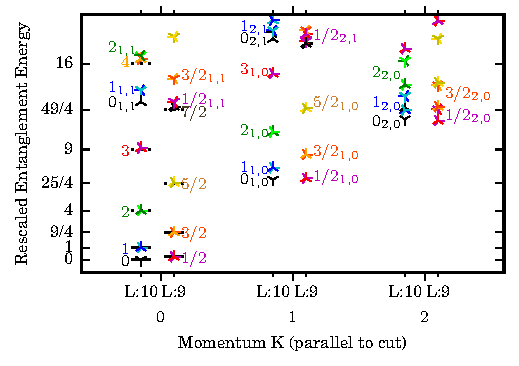
\includegraphics[width=\columnwidth]{EEIdentify.pdf}
	\caption{The identification of the primary states $\ket{\pm e, m=0}$ and the level $n, \bar{n}$ 
	descendants in the spectrum of the soft-core boson entanglement Hamiltonian. The states are labeled 
	$e_{n, \bar{n}}$. The zero and scale of the numerical spectrum are set by matching the lowest two 
	states. The energies and charges of the primaries with charges $2, 5/2, ... 4$ appear at the predicted 
	spots.  The best estimate for the Luttinger parameter from this spectrum is $\kappa \approx 1/6.4$, 
	taken from the energy of the $0_{1, 0}$ state. }
	\label{fig:EEIdentify}
\end{figure}

We can also take the lowest-lying Schmidt state, interpret it as the 
ground state of a 1d Hamiltonian, and consider its entanglement.

\begin{figure}[htbc]
	\centering
	\includegraphics[width=\columnwidth]{{EdgeGS_EntanglementEntropy.pdf}}
	\caption{Entanglement entropy within the entanglement ground state 
of the soft-core boson state on $10$ sites. For comparison, the 
Cardy-Calabrese formula $S(x) = c/3 \log \sin( \pi x/L) + const.$ is 
shown with $c=\frac{1}{2}, 1,$ and $2$, with the $const.$ fixed by 
matching the maximum of the entanglement entropy data. $c=1$ is a good 
fit.}
	\label{fig:EdgeGS_EE}
\end{figure}